
%% FAZIT %% 
\chapter{Evaluation}
In the Evaluation chapter, the system usability is checked with the help of the system usability scale (SUS). The extent to which the system requirements have been met is considered aftward. For the reasons already mentioned, the evaluation of the correctness of the diagnoses is not carried out in this work.

\section{System Usability Scale}
The SUS makes it possible to determine the usability of an application using a questionnaire \cite{.sus}. The application is currently still in an early stage of development, as the focus was on the conception and possible implementation during the work. The questions are asked based on graphical interfaces. The following questions  \cite{.sus} are asked of anonymous persons:
\begin{figure}[H]
	\centering
	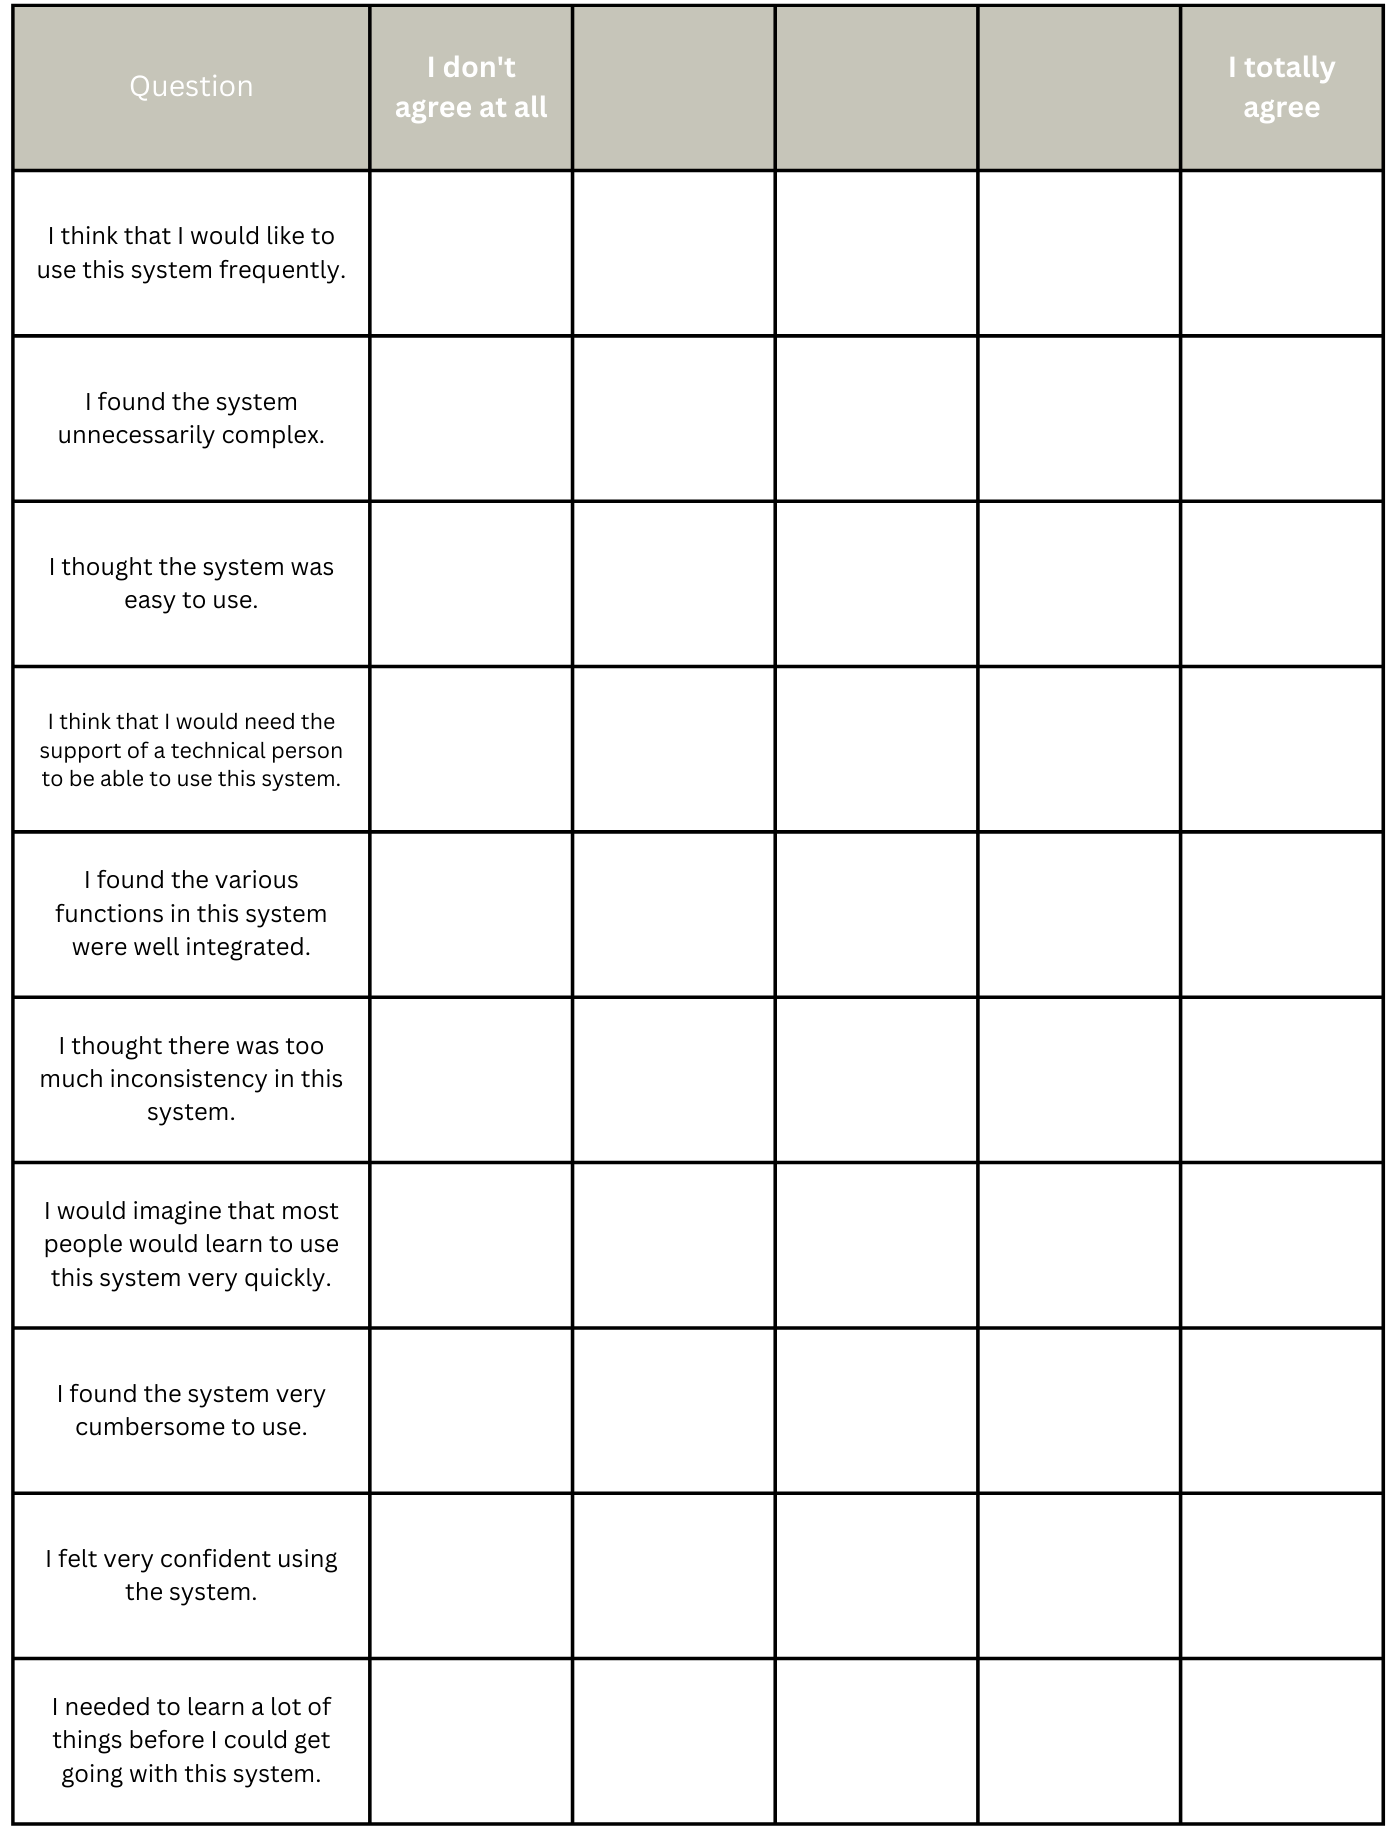
\includegraphics[scale=0.25]{SUS Template.png}
	\caption{SUS Template}
\end{figure}
\subsubsection{Evaluation of the SUS}
The possible answers are given values from 0 to 4, where 0 equals "I do not agree at all". Based on that, the following values are the result:
\begin{figure}[H]
	\centering
	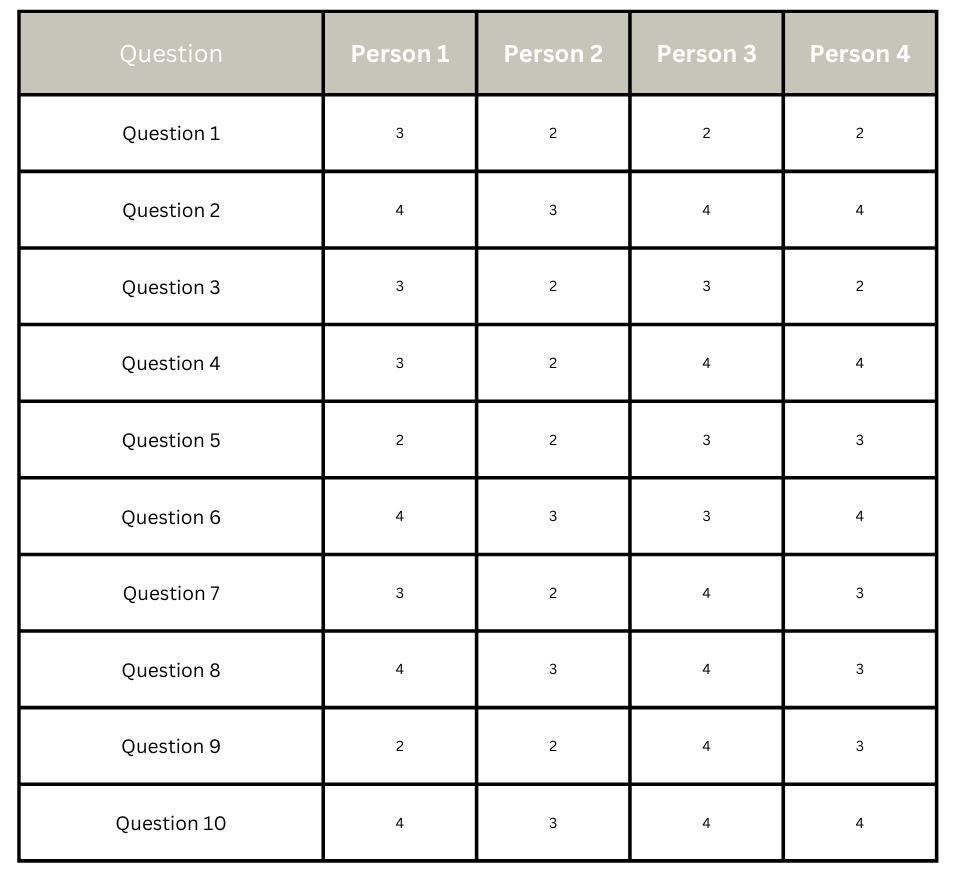
\includegraphics[scale=0.4]{susanswers.png}
	\caption{SUS Answers}
\end{figure}
\noindent
The SUS score is calculated as described in \cite{.sus} (all answers are added up and multiplied by 2,5). The following values are created for the individual persons:
\begin{itemize}
	\item Person 1: 80 \%
	\item Person 2: 60 \%
	\item Person 3: 87,5 \%
	\item Person 4: 80 \%
\end{itemize}
Altogether this results in a SUS score of 76.875\%. This can be rated as above average \cite{.sus}, and the usability of the system, based on the current design status, can be considered satisfactory.
\section{Requirements}
\begin{itemize}
	\item \textbf{[OR1]: The application should make it possible to save and download a diagnosis in PDF format}
	\newline
	This requirement can be fulfilled as described in chapter 7.5.2.
	\item \textbf{[OR2]: The application should make it possible for a user to save tips on a favorites list}
	\newline
	Similar to the methodology of how diagnoses are stored in the system, it is also possible to store advice. These also get their own class whose instances can be stored in a list and using methods described in 7.5.2, and the data is converted and stored as shown in Listing 7.3.
	\item \textbf{[FR1]: The application must allow the user to switch between the diagnostics and the advice view}
	\newline
	Switching between screens can be implemented via the described AppNavigator. 
	\item \textbf{[FR2]: The application must offer the user the option of being able to verify themselves as a doctor, and [FR3]: The application must offer a doctor the opportunity to log in}
	\newline
	The steps taken for this were described in detail in Chapter 7.5.1. However, it should be noted that another method should be used for the verification of doctors.
	\item \textbf{[FR4] and [FR5]: The application must offer a doctor the opportunity to add a new record in the database and to edit old datasets}
	\newline
	The data models described in Chapter 7.2 are used to enable the doctors to do this. The doctor can use this to create new objects and add them to the database using the DatabaseService described in Chapter 7.1. The database service also ensures that the already available data is displayed to the doctor and can be edited.
	\item \textbf{[FR6]: The application must allow a user to start a new diagnosis}
	\newline
	This is done by clicking on the button provided for this purpose on the start page, which has also been marked with suitable text.
	\item \textbf{[FR7]: The application must enable a user to save a diagnosis}
	\newline
	This requirement can also be met using the methodology described in 7.5.2.
	\item \textbf{[FR8]: The application must enable a user to view his saved diagnoses again}
	\newline
	By accessing the data entries stored in the SharedPreferences, the system can access the associated key and display the data accordingly on the screen.
	\item \textbf{[FR9]: The application must allow a user to abort his diagnostic procedure at any time, and [FR11]: The application must allow a doctor to abort adding or editing data at any time}
	\newline
	This is given by clicking on the "back" button. This is displayed to the user throughout the whole process.
	\item \textbf{[FR10]: The application must allow a user to delete saved diagnoses}
	\newline
	SharedPreferences allows it to access and delete saved data.
	\item \textbf{[NFR1]: The application must make correct diagnoses}
	\newline
	In the context of this work, this requirement cannot be met because there needs to be correct data for the calculation. As already mentioned, dummy data was used here.
	\item \textbf{[NFR2]: The application must be usable for patients without registration}
	\newline
	This is ensured because the user can access all the views he needs without restrictions since none have been integrated. Only the Doctor Panel has to be blocked for users who are not verified and logged in using the login mechanism.
	\item \textbf{[NFR3]: The application should have a graphical interface that can be used intuitively}
	\newline
	The results from the second survey show that the graphical interface is generally intuitive to use.
\end{itemize}
In general, most requirements can be implemented. The use of the Flutter framework, in particular, allows an easy implementation.




\chapter{Conclusion and Outlook}
Based on the growth of interest regarding health issues and the contexts of busy medical practices discussed, this work was generated as a template for current and future medical apps.
The aim of the present work, "Development of a mobile application for the algorithmic attribution of symptoms to potential diseases," was to design a smartphone application for the described situation, generate first development ideas with the framework Flutter, and evaluate the generated results. The main aim was to design a platform to relieve doctors' offices' burden and calm worried patients. 
\newline \\
Using the personas, the requirements and the use cases that can occur during the application use could be determined. The survey conducted at the work's initial stage also helped obtain more precise information on non-functional and functional requirements. In the context of this work, it made sense to interact with the potential user group at an early stage and to involve them in the development and planning process. However, doctor verification should be discussed in the future. As part of the bachelor thesis, only the possibility of e-mail verification was discussed. However, this should not be used in the real world since any user could do this, even if he is not a doctor. One possibility would be to provide manual verification, which allows the app developers themselves, or a designated authority, to create and verify doctor accounts. In cooperation with the proper authorities, it can be ensured that only the right people have access to the medical area.
\newline \\
A positive aspect during the processing was that almost all functional and optional requirements can be fulfilled. The Flutter framework is helpful here, as many functionalities can be implemented with fewer lines of code thanks to the wide range of dependencies.
\newline \\
By determining the system context, it could be recognized that an external API will also affect the system. In the following, two different APIs were evaluated, and a decision was made. In the following, the choice of the ApiMedic API made sense for this work. However, it should be considered in the future whether to scrape the data from the NHS API. These turn out to be more detailed and could lead to a more detailed application. On the other hand, the database should be expanded with data sets created by doctors. 
\newline \\
With the generated domain model and the API data, classes for implementation could already be generated, and a database structure determined. For a simplified representation within this work, only the names were used as IDs for the Firestore database documents. In reality, however, this is not recommended. A hash functionality would be more suitable to ensure that nobody outside can manipulate the diseases and symptoms. The classes created and the structuring of the project, which was carried out in Chapter 6, help implement clean design principles, such as the SOLID principles.
\newline \\
As part of the first survey mentioned, it was found that the application's graphical user interface plays an important role. Accordingly, design principles were considered and created based on these first conception ideas. These were equipped with implementation proposals for Flutter. Subsequently, mock-ups could already be generated. These were evaluated in a second survey for their user-friendliness and intuitiveness. The design solutions provided are rated as intuitive by the respondents. As part of an analysis using SUS, it was also found that the graphical user interface is above average in terms of usability. Concerning the diagnosis process, the graphical user interface could be improved. Users are forced to select their body parts and symptoms by scrolling through large lists. It would be possible to simplify this using a search bar. However, the user would have to know the name of his symptom for this, which proves to be difficult with technical terms. For this reason, the search algorithm must be expanded to the extent that it can also assign related terms.
\newline \\
A similar search facility should also be made available to doctors to assist them in their search for specific symptoms and diseases.
\newline \\
Finally, possible algorithmic solutions for the implementation of the diagnosis were compared. Whether the chosen algorithm has a high correctness rate could not be determined. A bad point, however, was that the time it took to perform the calculation was too high for an average user, even though the CPU usage turned out to be low. This long calculation time can probably also be attributed to the queries to the database since these can also be time-consuming with a large number of queries. Regarding the algorithm, the dummy data with which the application is currently working should be replaced with actual data. It is also urgently necessary to optimize the calculation time. Here one can think about describing symptoms in more detail. For example, the user could be asked questions about their reported symptoms, and possible causes (e.g., not drinking enough, not sleeping, medications the patient is taking, ...). Based on these selections, certain diseases may be excluded in advance while others gain in importance. In addition, medical professionals should be consulted to ensure the correctness of the diagnoses. 
\newline \\
\textbf{In general, it can be said that a user-friendly application can be developed using the approaches discussed. However, improvements should be made regarding the performance of disease detection. It is not possible to predict whether a change in the data structure will be necessary for this.}
%\section{Symptom Detection Applications in the Future}
%\section{Overall Conclusion}

